% 05_material.tex
\chapter{Material selection}\label{sec:material}

The material was chosen by an open trade study over the filaments the P1S can print, with the selected filament then assumed bought. The study follows the usual sequence of materials selection~\citep{ashby}: translate the design requirement into a merit index, remove the candidates that fail a hard limit, rank the rest by the index, and check the ranking against independent data before trusting it.

\section{Merit index for a stiffness-limited arm}\label{sec:material-index}

\Cref{sec:requirements,sec:loads} established that the frequency requirement, not strength, sizes the arms. The index follows from that, step by step.

\paragraph{What the arm must do.} With the motor and propeller as a tip mass $m_\text{tip}$ on a cantilever of free length $L$, the first bending frequency is
\begin{equation}
f = \frac{1}{2\pi}\sqrt{\frac{k}{m_\text{tip}}},
\end{equation}
so a frequency target fixes the tip stiffness:
\begin{equation}
k = (2\pi f)^2\, m_\text{tip}.
\end{equation}
The target and the tip mass are fixed, so $k$ is fixed, and every material must reach the same $k$.

\paragraph{How the arm makes that stiffness.} For a cantilever loaded at its tip,
\begin{equation}
k = \frac{3EI}{L^3},
\end{equation}
and for a rectangular section of width $b$ and height $h$,
\begin{equation}
I = \frac{bh^3}{12}.
\end{equation}
Substituting:
\begin{equation}
k = \frac{Ebh^3}{4L^3}.
\end{equation}

\paragraph{What is fixed and what is free.} The layout sets $L$. The width $b$ is held small, because every millimetre of width costs flight time through download (\cref{sec:sizing-width}). The height $h$ is free: it costs mass but no download. Each material therefore reaches the required $k$ with its own height. Solving for $h$:
\begin{equation}
h = \left(\frac{4kL^3}{Eb}\right)^{1/3}.
\end{equation}
With $k$, $L$ and $b$ fixed, $h$ grows as $E^{-1/3}$: a stiffer material needs a shallower arm, but only by the cube root.

\paragraph{What that costs in mass.} The arm's mass is
\begin{equation}
m = \rho\, b\, h\, L.
\end{equation}
Substituting $h$:
\begin{equation}
m = \rho\, b\, L \left(\frac{4kL^3}{Eb}\right)^{1/3}.
\end{equation}
Everything except $\rho$ and $E$ is the same for every material, so
\begin{equation}
m \propto \rho\, E^{-1/3}.
\end{equation}

\paragraph{The index.} The lightest arm comes from the material with the smallest $\rho E^{-1/3}$, which is the same as the largest
\begin{equation}
M = \frac{E^{1/3}}{\rho}.
\end{equation}
This is Ashby's index for a stiffness-limited beam whose width is fixed and whose height is free. Density counts in full, while modulus counts only through its cube root: a material twice as stiff makes the arm only 21\,\% shallower, because $2^{-1/3} = 0.79$. The index also depends on the constraint. A beam free to scale in both width and height would use $E^{1/2}/\rho$; holding the width small is what makes density dominate here. The index assumes a solid rectangular section with the frequency set by the tip mass. The optimised truss or ribbed section changes the absolute masses, but not the ranking between materials.

\section{Candidates and gates}\label{sec:material-gates}

The candidates are the eight filaments with complete technical data sheets from one manufacturer~\citep{bambu_tds}: PLA Basic, PLA-CF, PETG HF, PETG-CF, ASA, PET-CF, PAHT-CF and PPA-CF, all tested dry, at 100\,\% infill, with separate specimens printed in the layer plane ($xy$) and across the layers ($z$). TPU 95A HF was considered only for flexible parts.

Two gates remove candidates before any ranking.
\begin{itemize}
\item \textbf{Heat} (R5): heat deflection temperature at \SI{0.45}{MPa} of at least \SI{70}{\celsius}. The motors heat their mounts, and a frame that creeps at the motor pads loses its alignment. The motor-mount temperature after hard flights was not measured; \SI{60}{\celsius} is assumed, with a \SI{10}{\celsius} margin. The gate removes PLA (\SI{57}{\celsius}), PLA-CF (\SI{55}{\celsius}) and PETG HF (\SI{69}{\celsius}).
\item \textbf{Printability on the P1S}: PPA-CF needs a nozzle of 280 to \SI{310}{\celsius} against the printer's maximum of \SI{300}{\celsius}, and a heated chamber of 50 to \SI{80}{\celsius} that the P1S lacks. All carbon-fibre grades need a hardened steel nozzle.
\end{itemize}

\begin{figure}[htbp]
\centering
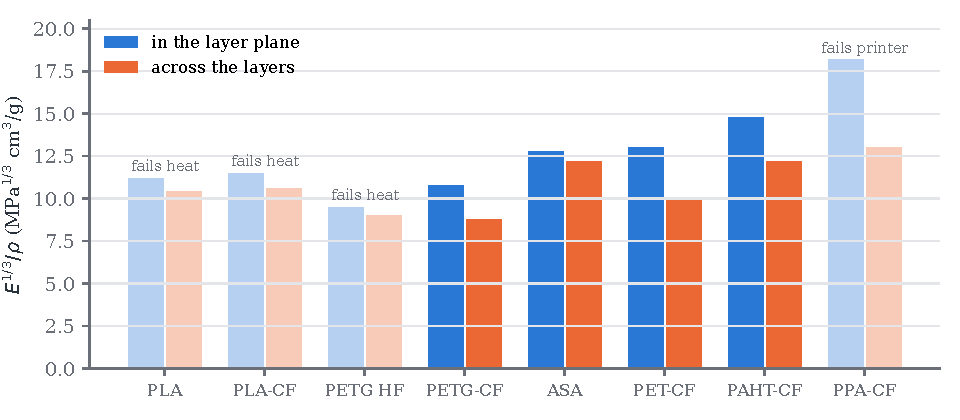
\includegraphics[width=0.95\linewidth]{plot_merit}
\caption{Frequency merit index of the candidates from manufacturer data, in the layer plane and across the layers. Pale bars fail a gate.}\label{fig:material-merit}
\end{figure}

\begin{table}[htbp]
\centering\small
\caption{Survivors of the gates, ranked by the merit index in the layer plane (manufacturer data). Arm mass is relative to a PLA arm of the same frequency.}\label{tab:material-ranking}
\begin{tabular}{@{}lccccc@{}}
\toprule
Material & Index $xy$ ($z$) & Arm mass & Strength $z$ (MPa) & Impact $z$ (kJ/m$^2$) & HDT (\si{\celsius})\\
\midrule
PAHT-CF & 14.8 (12.2) & 0.76 & 64 & 13.3 & 194\\
PET-CF & 13.0 (10.0) & 0.86 & 38 & 4.5 & 205 annealed\\
ASA & 12.8 (12.2) & 0.87 & 31 & 4.9 & 100\\
PETG-CF & 10.8 (8.8) & 1.04 & 38 & 10.7 & 74\\
\bottomrule
\end{tabular}
\end{table}

On manufacturer data PAHT-CF leads (\cref{fig:material-merit,tab:material-ranking}): the best index, the best across-layer strength and the best impact resistance. ASA has a low density and nearly isotropic stiffness but is brittle across layers and warps. PETG-CF is easy to print but marginal on the heat gate and the heaviest arm of the four.

\section{Anisotropy of printed material}\label{sec:material-anisotropy}

A printed part is a stack of layers, each made of extruded lines. Inside a line the polymer, and the short fibres it carries, are continuous and aligned with the print path; between lines and between layers the material is bonded only where the hot extrudate fused to the cold one beneath it. Across the layers ($z$) the data sheets give 46 to 87\,\% of the in-plane stiffness, 50 to 90\,\% of the in-plane strength, and only 10 to 52\,\% of the impact energy.

Coupon tests by the author on PLA (printed flat on a Bambu X1C, with rasters at \ang{0} and \ang{90} to the specimen axis) show the same pattern within a layer. Loading across the rasters lowered the modulus only slightly (2660 to \SI{3000}{MPa} against 2660 to \SI{3530}{MPa} along them) and the strength more (30 to \SI{43}{MPa} against 40 to \SI{59}{MPa}), and it cut the Charpy energy by roughly three to five times (0.08 to \SI{0.28}{J} against 0.36 to \SI{0.91}{J}). Impact across rasters and layers is the weakest property of every printed material. It steers the print orientation, which puts the bending stresses of the arms in the layer plane, and it is one reason the crash case is handled by a defined failure order instead of by strength.

\section{Independent data}\label{sec:material-independent}

Manufacturer data sheets may present their materials favourably, so the shortlist was checked against standardised independent tests of in-plane tensile strength and layer adhesion~\citep{mytechfun_siraya} (\cref{tab:material-independent}).

\begin{table}[htbp]
\centering\small
\caption{Manufacturer against independent strengths.}\label{tab:material-independent}
\begin{tabular}{@{}lcccc@{}}
\toprule
& \multicolumn{2}{c}{In the layer plane (MPa)} & \multicolumn{2}{c}{Across the layers (MPa)}\\
\cmidrule(lr){2-3}\cmidrule(l){4-5}
Material & sheet & independent & sheet & independent\\
\midrule
PAHT-CF (Bambu) & 88 & 67.4 & 64 & 20\\
PET-CF (Bambu) & 74 & 69 & 35 & 28.5\\
PET-CF (Siraya Fibreheart) & 74 & 64 & 35 & 28.1\\
\bottomrule
\end{tabular}
\end{table}

The across-layer strength of PAHT-CF on its data sheet, \SI{64}{MPa}, is three times the independent value of \SI{20}{MPa}. Both PET-CF grades agree with their sheets within about 20\,\%. PAHT-CF loses its main advantage, and it adds the drying a nylon needs (80\,\textdegree C for 8 to 12 hours) and the moisture sensitivity of its properties.

\section{Choice and design values}\label{sec:material-choice}

Siraya Tech Fibreheart PET-CF, a PET with 15\,\% short carbon fibre, printed unannealed, was chosen~\citep{siraya_petcf}. Its frequency index is 13.9 in the layer plane and 11.6 across the layers on its own data sheet. It passes the heat gate without annealing, with a heat deflection temperature of \SI{86.7}{\celsius} at \SI{0.45}{MPa}, so the distortion that annealing can cause is avoided. It costs \SI{40}{EUR/kg} against \SI{90}{EUR/kg} for the other PET-CF grade, and it prints at 280 to \SI{300}{\celsius} with a hardened nozzle. Its moduli were measured to ASTM D638 and the other grades' to ISO 527, so part of its 26 to 57\,\% higher moduli may come from the test method and the specimens.

The design values take the data-sheet moduli and the independent strengths, each multiplied by 0.85 for scatter and print settings (\cref{tab:material-design}).

\begin{table}[htbp]
\centering\small
\caption{Design values for Siraya Fibreheart PET-CF, unannealed.}\label{tab:material-design}
\begin{tabular}{@{}lccc@{}}
\toprule
Property & Source value & Design value ($\times 0.85$) & Allowable / 1.5\\
\midrule
$E_{xy}$ & \SI{5950}{MPa} & \SI{5058}{MPa} & \\
$E_z$ & \SI{3400}{MPa} & \SI{2890}{MPa} & \\
$S_{xy}$, tensile & \SI{64}{MPa} & \SI{54.4}{MPa} & \SI{36.3}{MPa}\\
$S_z$, layer adhesion & \SI{28.1}{MPa} & \SI{23.9}{MPa} & \SI{15.9}{MPa}\\
Density & \SI{1.30}{g/cm^3} & \SI{1.30}{g/cm^3} & \\
\bottomrule
\end{tabular}
\end{table}

No compressive or shear strengths exist for this material. Compression is taken equal to tension, which is conservative for fused-filament parts, where compressive strength is usually higher; shear between layers is checked against the layer adhesion strength, an assumption stated with the strength check.

\section{Material model}\label{sec:material-model}

Every part is printed with its layers in the global $xy$ plane, so the material is modelled as transversely isotropic with the build direction along $z$: one set of properties in the layer plane, another across it. Neither the data sheet nor the independent tests give Poisson's ratios or shear moduli. The model takes $\nu = 0.35$, inside the 0.2 to 0.4 reported for fused-filament materials, and derives the shear moduli from the isotropic relation in each plane:
\begin{equation}
G_{xy} = \frac{E_{xy}}{2(1+\nu)} = \frac{5058}{2.7} = \SI{1873}{MPa}, \qquad G_{xz} = G_{yz} = \frac{E_z}{2(1+\nu)} = \frac{2890}{2.7} = \SI{1070}{MPa}.
\end{equation}
The error this assumption can cause is small. A Timoshenko beam model of the arm attributes 13\,\% of its tip deflection to shear, and changing $G$ from 700 to \SI{1500}{MPa} moves its first frequency from 665 to \SI{700}{Hz}, $-3$ to $+2$\,\% around the \SI{687}{Hz} of the nominal value, well inside the margin of the frequency goal.

\section{Flexible parts and cost}\label{sec:material-cost}

The retainers that hold the receiver, the GPS and the antenna, and the skid on the floor of the body, are printed in TPU 95A HF, a thermoplastic polyurethane whose flexibility allows snap fits and press fits, and whose impact and abrasion resistance suits a sacrificial landing surface. They are not part of the optimised structure.

At 20 to \SI{100}{EUR/kg}, a frame of about \SI{60}{g} costs roughly 1 to \SI{6}{EUR} of filament for any candidate, against \SI{37.91}{EUR} for the reference frame. Cost does not discriminate between the candidates; the frame meets R9 whichever filament is chosen.
